\documentclass[12pt, a4]{article}
\usepackage[english]{babel}
\usepackage[utf8x]{inputenc}
\usepackage{fullpage}
\usepackage{listings}
\usepackage{graphicx}
\usepackage{color}

%Syntax highlighting
\definecolor{blue-violet}{rgb}{0.54, 0.17, 0.89}
\definecolor{ao}{rgb}{0.0, 0.5, 0.0}
\definecolor{amaranth}{rgb}{0.9, 0.17, 0.31}
\definecolor{ballblue}{rgb}{0.13, 0.67, 0.8}
\definecolor{onyx}{rgb}{0.06, 0.06, 0.06}


\lstset{
  breaklines=true,                 % automatic line breaking only at whitespace
  captionpos=b,                    % sets the caption-position to bottom
  breakatwhitespace=false,
  keepspaces=true,
  numbers=left,
  numbersep=5pt,
  showspaces=false,
  showstringspaces=false,
  showtabs=false,
  tabsize=4,  
  backgroundcolor=\color{white},   % choose the background color
  commentstyle=\color{ao},    % comment style
  keywordstyle=\color{amaranth},    % keyword style
  stringstyle=\color{blue-violet},    % string literal style
  numberstyle=\tiny\color{ballblue},	   % number style
  basicstyle=\ttfamily\footnotesize\color{onyx} % size of fonts used for the code
}

%Document Header
\title{\textbf{Department of CSE\\SSN College of Engineering}}
\author{\textbf{Vishakan Subramanian - 18 5001 196 - Semester VII}}
\date{17 October 2021}

\begin{document}
\maketitle
\hrule
\section*{\center{UCS 1712 - Graphics And Multimedia Lab}}
\hrule
\bigskip

%Assignment Details
\subsection*{\center{\textbf{Exercise 9: 3-Dimensional Projections in C++ using OpenGL}}}
\subsection*{\flushleft{Aim:}}
\begin{flushleft}

Write a menu driven program to perform Orthographic parallel projection and Perspective projection on any 3D object.
\bigskip

Set the camera to any position on the 3D space. Have $(0, 0, 0)$ at the center of the screen. Draw X, Y and Z axis. You can use gluPerspective() to perform perspective projection.

\bigskip

Use keyboard functions to rotate and show different views of the object. 

\bigskip
\textbf{Note:} Can use built-in functions for 3D transformations.
 
\end{flushleft}

%Code
\newpage
\subsection*{\flushleft{Code: 3D Projections:}}
\begin{flushleft}
\lstinputlisting[language = C++]{Projections.cpp}
\end{flushleft}


%Output
\newpage
\subsection*{\flushleft{Output: 3D Object - Ortho}}
\begin{figure}[h]
\centering
\caption{3D Object - Ortho.}
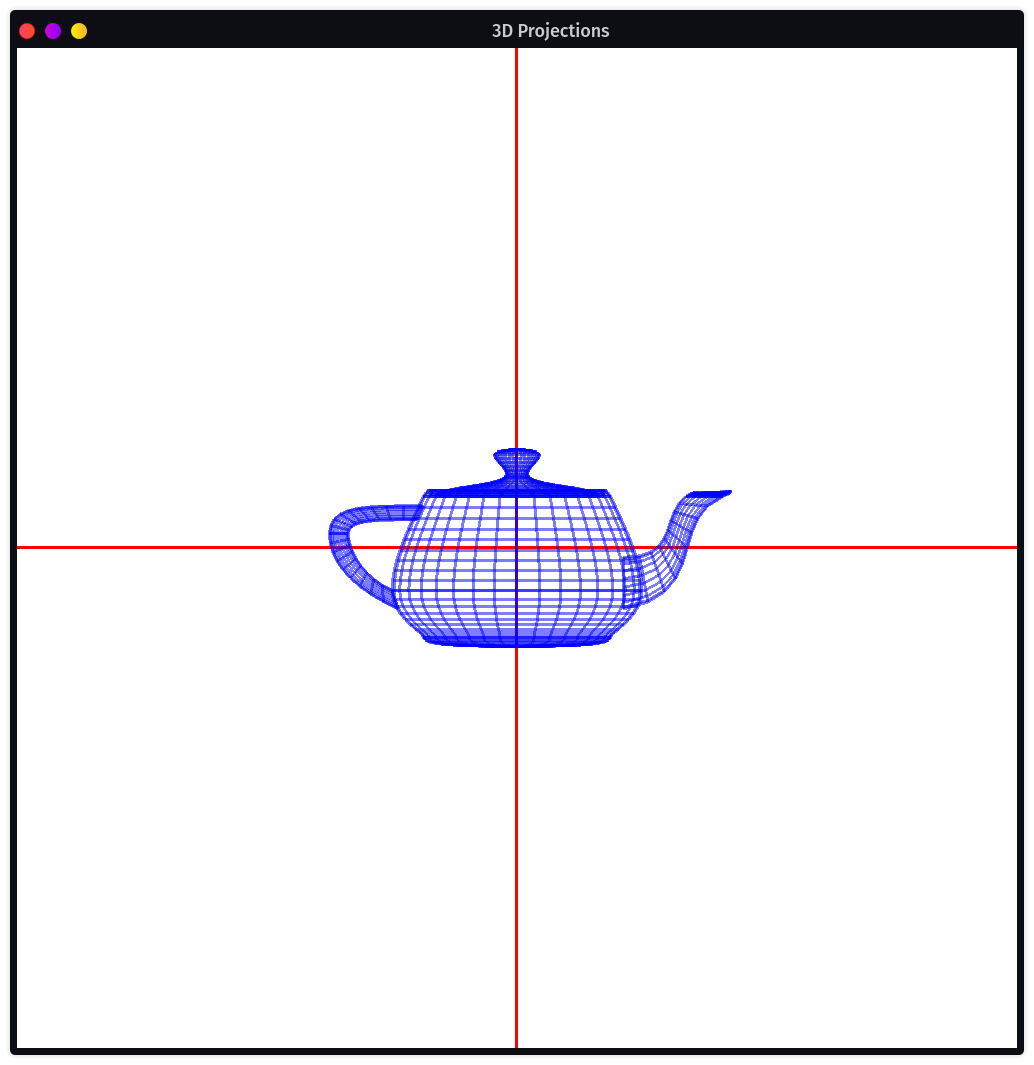
\includegraphics[height=15cm, width=15cm]{Outputs/Ortho1.png}
\end{figure}

%Output
\newpage
\subsection*{\flushleft{Output: 3D Object - Perspective}}
\begin{figure}[h]
\centering
\caption{3D Object - Perspective.}
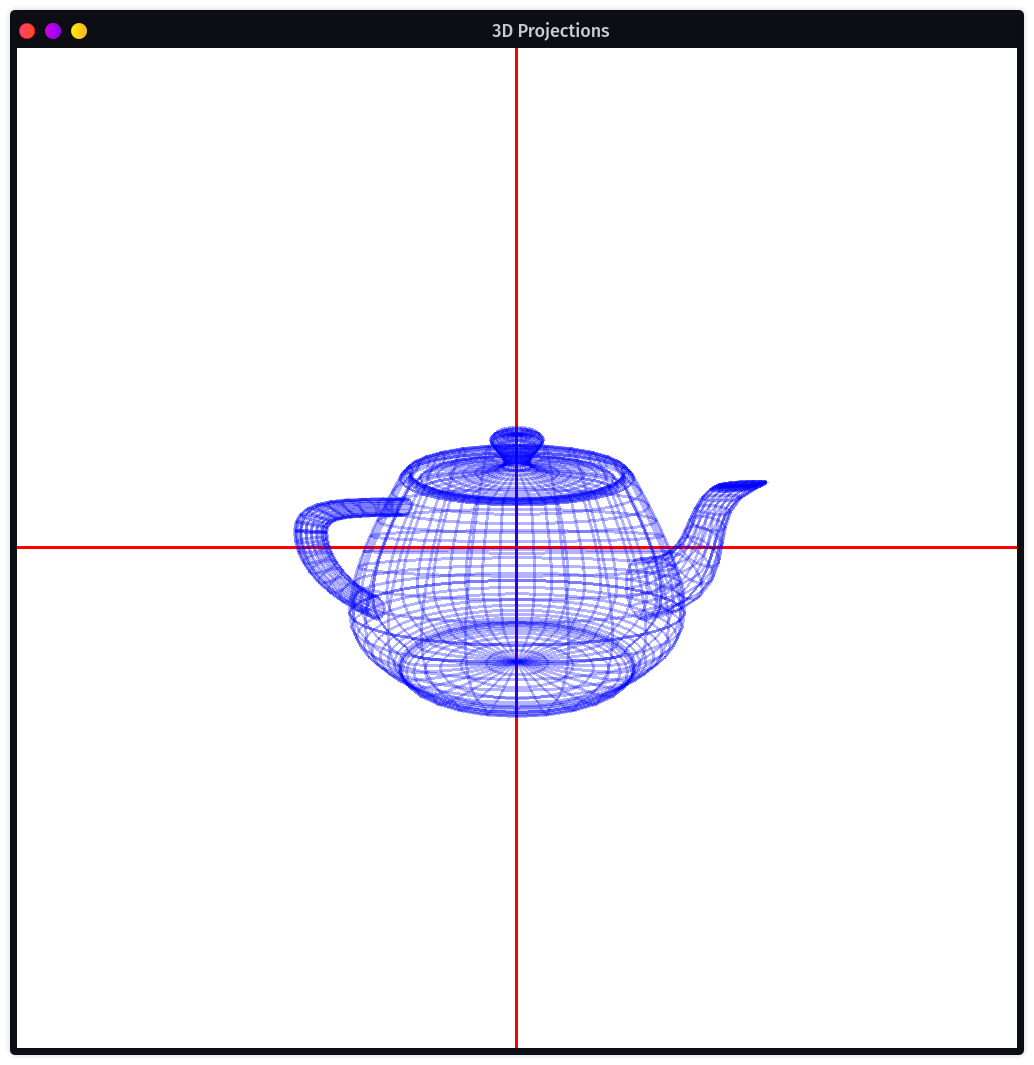
\includegraphics[height=15cm, width=15cm]{Outputs/Perspective1.png}
\end{figure}

%Output
\newpage
\subsection*{\flushleft{Output: 3D Object - Ortho (Rotated)}}
\begin{figure}[h]
\centering
\caption{3D Object - Ortho (Rotated).}
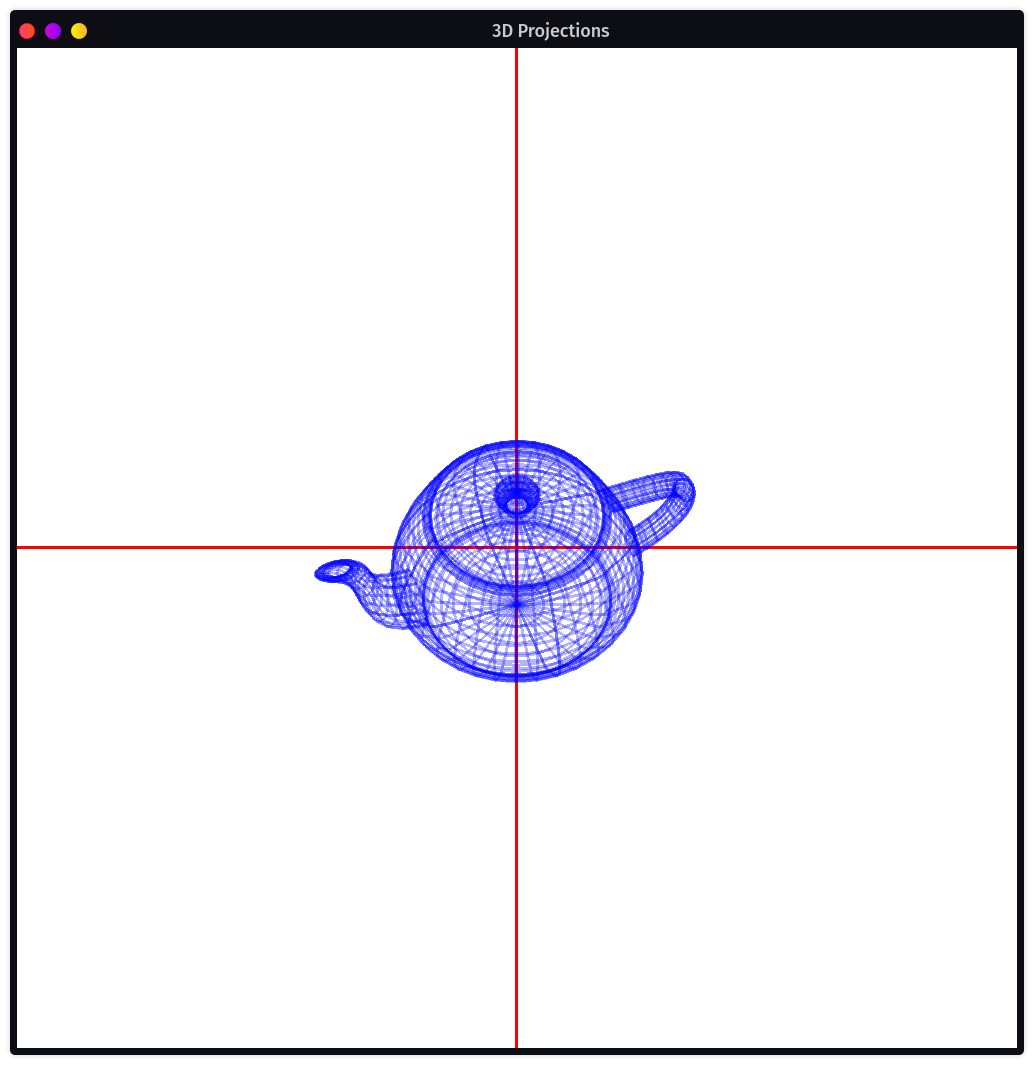
\includegraphics[height=15cm, width=15cm]{Outputs/Ortho2.png}
\end{figure}

%Output
\newpage
\subsection*{\flushleft{Output: 3D Object - Perspective (Rotated)}}
\begin{figure}[h]
\centering
\caption{3D Object - Perspective (Rotated).}
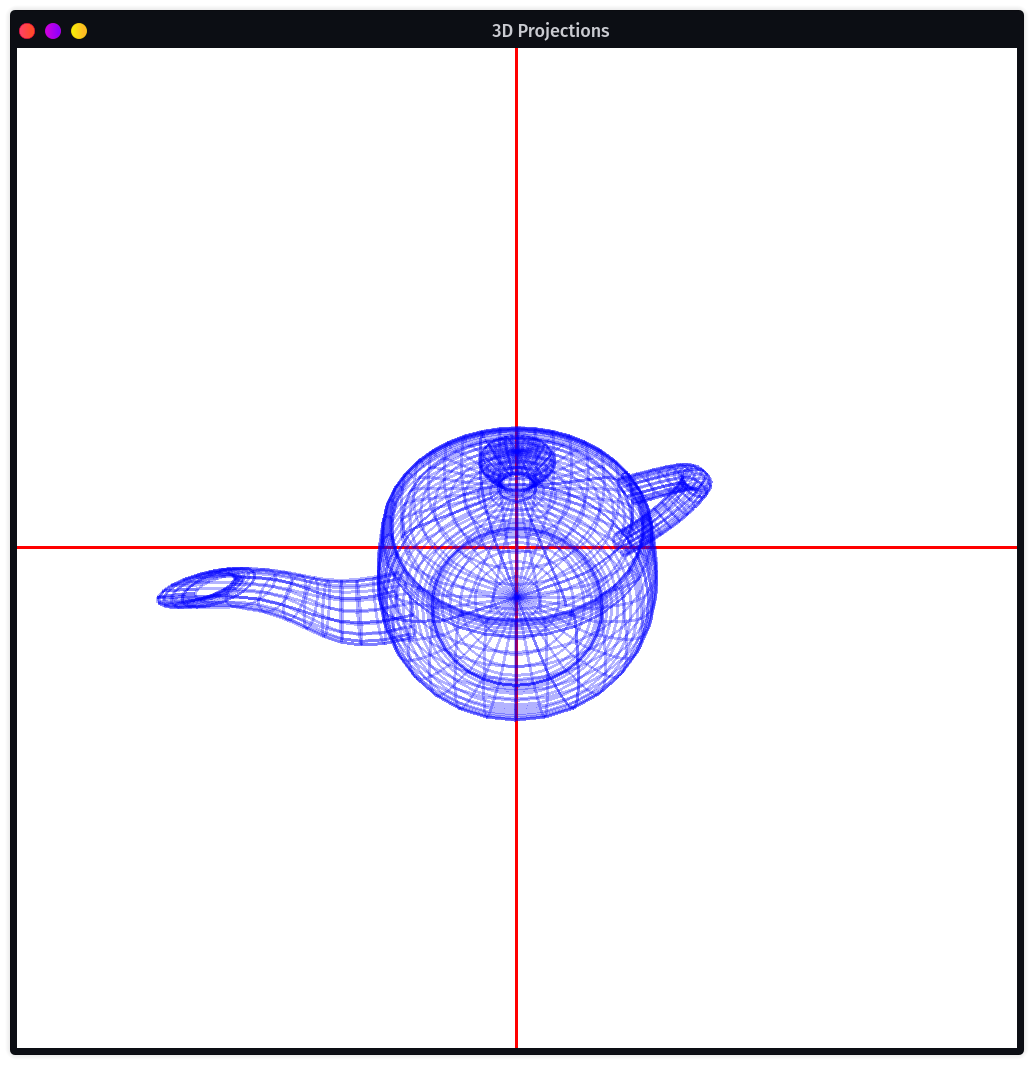
\includegraphics[height=15cm, width=15cm]{Outputs/Perspective2.png}
\end{figure}


%Learning Outcome
\newpage
\subsection*{\flushleft{Learning Outcome:}}
\begin{itemize}
\item I learnt how to set-up \textbf{keyboard functions} for handling different user inputs for rotation \& projections using \textbf{glutKeyboardFunc()} callback method.
\item I learnt how to use inbuilt 3D transformation methods like \textbf{glRotatef() and glTranslatef()}.
\item I understood the working of \textbf{glOrtho() and gluPerspective()} methods.
\item I learnt how to set-up camera position using \textbf{gluLookAt()} method.
\item I understood the usage of \textbf{glPushMatrix() \& glPopMatrix()}.
\item I understood the difference between the matrix modes of \textbf{GL\_MODELVIEW \& GL\_PROJECTION}, and when to use which.
\item I was able to use the inbuilt \textbf{glutWireTeapot()} method to display a 3-D Teapot object and performed parallel and perspective projections upon them, apart from rotating the object in the X and Y directions.
\item I learnt about \textbf{field of view}, \textbf{aspect ratio} and how to properly configure \textbf{zNear \& zFar} in gluPerspective().
\item I learnt how orthographic and parallel projections differ from each other.
\item I understood how the \textbf{camera, center \& up vectors} are configured in gluLookAt().
\end{itemize}


\end{document}